\documentclass[11pt,a4paper]{article}
\usepackage{graphicx}
\usepackage{amsmath}
\usepackage{amssymb}
\usepackage{tcolorbox}
\usepackage{xcolor}
\usepackage{geometry}
\usepackage{tikz}
\usepackage{multicol}
\usepackage{array}
\geometry{margin=0.7in}

% Define colors
\definecolor{mlblue}{RGB}{31, 119, 180}
\definecolor{mlorange}{RGB}{255, 127, 14}
\definecolor{mlgreen}{RGB}{44, 160, 44}
\definecolor{mlred}{RGB}{214, 39, 40}
\definecolor{mlpurple}{RGB}{148, 103, 189}
\definecolor{mlgray}{RGB}{127, 127, 127}

\title{\LARGE\textbf{Discovery Worksheet}\\
\vspace{0.5em}
\Large Introduction to Machine Learning \& AI\\
\vspace{0.3em}
\large Discover the Patterns Before the Formulas}
\author{Machine Learning for Smarter Innovation\\
Week 0: Pre-Lecture Activity}
\date{}

\begin{document}
\maketitle

\begin{tcolorbox}[colback=mlblue!10, colframe=mlblue!70, title=How to Use This Worksheet]
\textbf{Important:} Complete this \textbf{BEFORE} attending the lecture!

\textbf{Your mission:}
\begin{itemize}
\item Look at the 6 charts (one per section)
\item Answer the discovery questions using calculations and observations
\item Find the patterns YOURSELF before hearing the technical terms
\item Compare answers with a partner (different answers are OK!)
\end{itemize}

\textbf{Time needed:} 75-90 minutes\\
\textbf{Materials:} Calculator, ruler, pencil
\end{tcolorbox}

\vspace{0.5em}

\begin{tcolorbox}[colback=mlorange!10, colframe=mlorange!70]
\textbf{Learning Philosophy:} You already understand these concepts from everyday life. This worksheet helps you discover the mathematical patterns behind what you already know intuitively. The lecture will then give you the formal language to describe your discoveries.
\end{tcolorbox}

\newpage

% ================================================================
% DISCOVERY 1: OVERFITTING
% ================================================================
\section*{Discovery 1: The Overfitting Paradox}

\begin{center}
\includegraphics[width=0.95\textwidth]{../charts/discovery_chart_1_overfitting.pdf}
\end{center}

\subsection*{Observe the Chart}

Three models are trying to predict house prices from square footage. All three were trained on the same blue dots (training data). Orange squares are NEW houses the models have never seen (test data).

\subsection*{Discovery Tasks}

\textbf{Task 1: Calculate Training Errors}

For each model, measure how far predictions are from the blue training points.

\begin{itemize}
\item Model A (red horizontal line): Approx. training error = \underline{\hspace{2cm}}
\item Model B (green curve): Approx. training error = \underline{\hspace{2cm}}
\item Model C (purple wiggly): Approx. training error = \underline{\hspace{2cm}}
\end{itemize}

Which model has the LOWEST training error? \underline{\hspace{4cm}}

\vspace{0.5em}

\textbf{Task 2: Calculate Test Errors}

Now measure how well each model predicts the NEW orange test points.

\begin{itemize}
\item Model A test error: \underline{\hspace{2cm}}
\item Model B test error: \underline{\hspace{2cm}}
\item Model C test error: \underline{\hspace{2cm}}
\end{itemize}

Which model has the LOWEST test error? \underline{\hspace{4cm}}

\vspace{0.5em}

\textbf{Task 3: The Paradox}

\begin{tcolorbox}[colback=mlred!10, colframe=mlred!70]
\textbf{Discovery Question:} \\
Model C has the BEST training performance but the WORST test performance!\\
Why does perfect training lead to poor testing?\\
\vspace{0.3em}
\underline{\hspace{14cm}}\\
\underline{\hspace{14cm}}\\
\underline{\hspace{14cm}}
\end{tcolorbox}

\textbf{Task 4: Plot the Trade-off}

On the grid below, plot training error (x-axis) vs test error (y-axis) for all three models:

\begin{center}
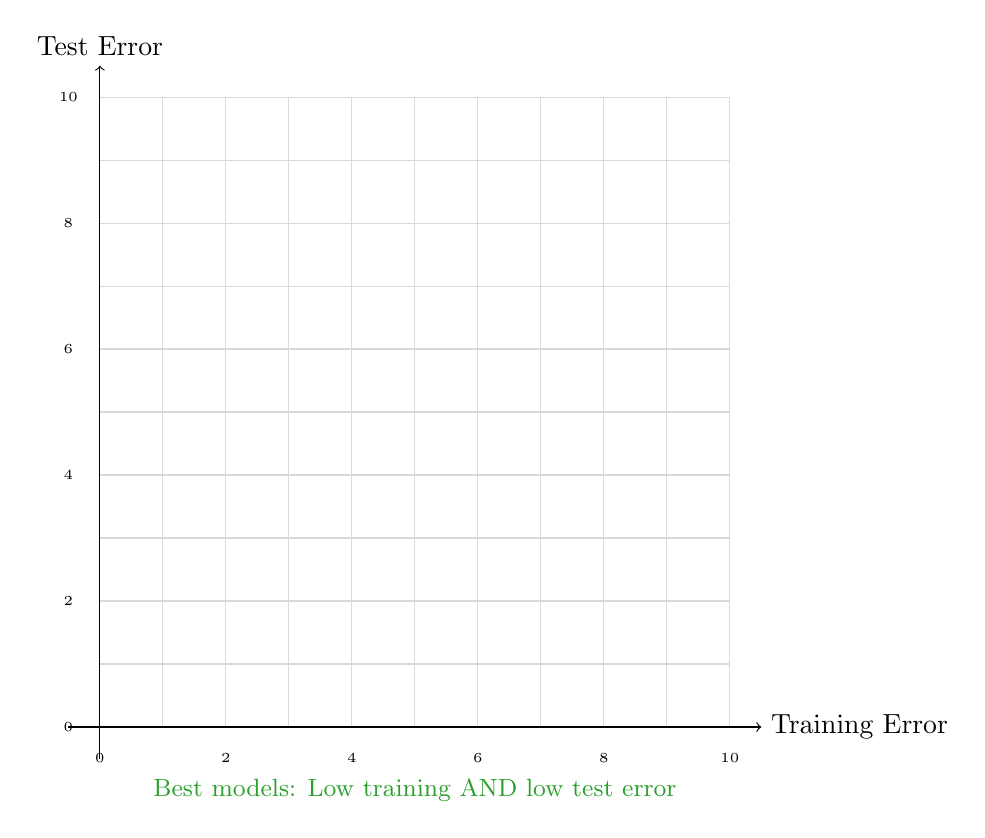
\begin{tikzpicture}[scale=0.8]
% Grid
\draw[gray!30, thin] (0,0) grid (10,10);
% Axes
\draw[->] (-0.5,0) -- (10.5,0) node[right] {Training Error};
\draw[->] (0,-0.5) -- (0,10.5) node[above] {Test Error};
% Numbers
\foreach \x in {0,2,4,6,8,10}
    \node at (\x,-0.5) {\tiny\x};
\foreach \y in {0,2,4,6,8,10}
    \node at (-0.5,\y) {\tiny\y};

% Hint: Ideal models are in bottom-left corner
\node[color=mlgreen] at (5,-1) {\small Best models: Low training AND low test error};
\end{tikzpicture}
\end{center}

What pattern do you see? \underline{\hspace{10cm}}

\vspace{0.5em}

\textbf{Task 5: Predict Model D}

Imagine Model D is even MORE complex than Model C (degree 20 polynomial).

\begin{itemize}
\item Predicted training error: \underline{\hspace{2cm}} (Why? \underline{\hspace{5cm}})
\item Predicted test error: \underline{\hspace{2cm}} (Why? \underline{\hspace{5cm}})
\end{itemize}

\begin{tcolorbox}[colback=mlpurple!10, colframe=mlpurple!70]
\textbf{Key Insight:}\\
Model A problem: \underline{\hspace{6cm}} (too simple)\\
Model C problem: \underline{\hspace{6cm}} (too complex)\\
Model B achieves: \underline{\hspace{6cm}} (balanced)\\
\vspace{0.3em}
\textit{In the lecture, you'll learn these have names: Bias and Variance}
\end{tcolorbox}

\newpage

% ================================================================
% DISCOVERY 2: K-MEANS
% ================================================================
\section*{Discovery 2: The Moving Centers Algorithm}

\begin{center}
\includegraphics[width=0.95\textwidth]{../charts/discovery_chart_2_kmeans.pdf}
\end{center}

\subsection*{Observe the Chart}

Watch how three centers (marked with stars) move over 5 steps to find natural groups in the data.

\subsection*{Discovery Tasks}

\textbf{Task 1: Calculate Center Movements}

In Step 2, centers move to the average position of their assigned points.

Calculate the Red center position in Step 2:
\begin{itemize}
\item Red cluster points visible in Step 1: Count = \underline{\hspace{1cm}}
\item Approximate center coordinates: (\underline{\hspace{1cm}}, \underline{\hspace{1cm}})
\item Movement distance from Step 0 to Step 2: \underline{\hspace{2cm}} units
\end{itemize}

\vspace{0.5em}

\textbf{Task 2: Calculate Within-Cluster Variance}

Variance measures how spread out points are from their center.

For the Red cluster in Step 1:
\[
\text{Variance} = \frac{1}{n}\sum(\text{distance from point to center})^2
\]

Pick 3 visible red points and calculate:
\begin{itemize}
\item Point 1 distance to red center: \underline{\hspace{2cm}}
\item Point 2 distance to red center: \underline{\hspace{2cm}}
\item Point 3 distance to red center: \underline{\hspace{2cm}}
\item Average squared distance: \underline{\hspace{2cm}}
\end{itemize}

\vspace{0.5em}

\textbf{Task 3: Track Variance Reduction}

The chart shows total variance values at each step.

\begin{center}
\begin{tikzpicture}[scale=0.9]
\draw[->] (0,0) -- (11,0) node[right] {Step};
\draw[->] (0,0) -- (0,5) node[above] {Total Variance};
\foreach \x in {0,1,2,3,4,5}
    \node at (\x*2,-0.3) {\x};

% Students fill in from chart
\node at (5,4.5) {Fill in variance values from chart:};
\node at (5,4) {Step 0: \underline{\hspace{1.5cm}}};
\node at (5,3.5) {Step 1: \underline{\hspace{1.5cm}}};
\node at (5,3) {Step 2: \underline{\hspace{1.5cm}}};
\node at (5,2.5) {Step 5: \underline{\hspace{1.5cm}}};
\end{tikzpicture}
\end{center}

Is variance increasing or decreasing? \underline{\hspace{5cm}}

\vspace{0.5em}

\textbf{Task 4: Convergence Detection}

\begin{tcolorbox}[colback=mlgreen!10, colframe=mlgreen!70]
\textbf{Discovery Question:}\\
How do you know the algorithm has finished? What stops changing?\\
\vspace{0.3em}
\underline{\hspace{14cm}}\\
\underline{\hspace{14cm}}
\end{tcolorbox}

\textbf{Task 5: Discover the Rules}

By watching the 6-step sequence, you can figure out the algorithm!

\textbf{The algorithm repeats two rules:}

\textbf{Rule 1 (Assignment):} Each point \underline{\hspace{8cm}}

\vspace{0.3em}

\textbf{Rule 2 (Update):} Each center moves to \underline{\hspace{7cm}}

\vspace{0.5em}

\textbf{Task 6: What Gets Optimized?}

The algorithm is trying to minimize something. What?

The objective is to minimize: \underline{\hspace{8cm}}

\begin{tcolorbox}[colback=mlblue!10, colframe=mlblue!70]
\textbf{Key Insight:}\\
This ``dance'' has a name: \textbf{K-Means Clustering}\\
K = number of \underline{\hspace{4cm}}\\
Means = \underline{\hspace{6cm}} position\\
It minimizes \underline{\hspace{5cm}} within clusters
\end{tcolorbox}

\newpage

% ================================================================
% DISCOVERY 3: BOUNDARIES
% ================================================================
\section*{Discovery 3: The Impossible Separation}

\begin{center}
\includegraphics[width=0.95\textwidth]{../charts/discovery_chart_3_boundaries.pdf}
\end{center}

\subsection*{Observe the Chart}

Four datasets show red and blue points. Your task: separate them with the simplest possible rule.

\subsection*{Discovery Tasks}

\textbf{Task 1: Draw Linear Boundaries}

Using a ruler, draw the best straight line to separate red from blue in each dataset.

Count classification errors for each:
\begin{itemize}
\item Dataset A errors: \underline{\hspace{1cm}}/\underline{\hspace{1cm}} = \underline{\hspace{2cm}}\%
\item Dataset B errors: \underline{\hspace{1cm}}/\underline{\hspace{1cm}} = \underline{\hspace{2cm}}\%
\item Dataset C errors: \underline{\hspace{1cm}}/\underline{\hspace{1cm}} = \underline{\hspace{2cm}}\%
\item Dataset D errors: \underline{\hspace{1cm}}/\underline{\hspace{1cm}} = \underline{\hspace{2cm}}\%
\end{itemize}

Which dataset(s) CAN be perfectly separated with a straight line? \underline{\hspace{5cm}}

\vspace{0.5em}

\textbf{Task 2: Mathematical Proof (Dataset D - XOR Pattern)}

Any straight line has equation: $ax + by + c = 0$

Points are classified as:
\begin{itemize}
\item Red if $ax + by + c > 0$
\item Blue if $ax + by + c < 0$
\end{itemize}

Test the four corners of Dataset D:

\begin{center}
\begin{tabular}{|l|c|c|c|}
\hline
\textbf{Point} & \textbf{Actual Color} & \textbf{$ax + by + c$} & \textbf{Predicted Color} \\
\hline
(1,1) & Red & \underline{\hspace{2cm}} & \underline{\hspace{2cm}} \\
(1,9) & Blue & \underline{\hspace{2cm}} & \underline{\hspace{2cm}} \\
(9,1) & Blue & \underline{\hspace{2cm}} & \underline{\hspace{2cm}} \\
(9,9) & Red & \underline{\hspace{2cm}} & \underline{\hspace{2cm}} \\
\hline
\end{tabular}
\end{center}

\begin{tcolorbox}[colback=mlred!10, colframe=mlred!70]
\textbf{Proof by Contradiction:}\\
Assume (1,1) is Red: $a + b + c > 0$\\
Then (9,9) is Red: $9a + 9b + c > 0$ \\
But (1,9) is Blue: $a + 9b + c < 0$\\
And (9,1) is Blue: $9a + b + c < 0$\\
\vspace{0.3em}
Add last two inequalities: $(a+9b+c) + (9a+b+c) < 0$\\
Simplifies to: $10a + 10b + 2c < 0$\\
But we need: $9a + 9b + c > 0$ (for point (9,9) to be Red)\\
\vspace{0.3em}
\textbf{Contradiction!} No single line can separate XOR pattern.
\end{tcolorbox}

\textbf{Task 3: Nonlinear Solutions}

For Dataset C (circular pattern), what shape boundary works?

Boundary type: \underline{\hspace{4cm}}

Equation: $x^2 + y^2 = $ \underline{\hspace{2cm}}

\vspace{0.5em}

For Dataset D (XOR pattern), propose a solution using TWO lines:

Line 1: $x = $ \underline{\hspace{2cm}} (vertical)\\
Line 2: $y = $ \underline{\hspace{2cm}} (horizontal)

Combined rule: Point is Red if \underline{\hspace{8cm}}

\vspace{0.5em}

\textbf{Task 4: When Linearity Fails}

\begin{tcolorbox}[colback=mlpurple!10, colframe=mlpurple!70]
\textbf{Key Discoveries:}\\
Linear models work when: \underline{\hspace{8cm}}\\
Linear models fail when: \underline{\hspace{8cm}}\\
Solution for complex patterns: \underline{\hspace{7cm}}\\
\vspace{0.3em}
\textit{In the lecture, you'll learn how neural networks combine multiple lines to solve XOR}
\end{tcolorbox}

\newpage

% ================================================================
% DISCOVERY 4: GRADIENT DESCENT
% ================================================================
\section*{Discovery 4: The Optimization Landscape}

\begin{center}
\includegraphics[width=0.75\textwidth]{../charts/discovery_chart_4_gradient.pdf}
\end{center}

\subsection*{Observe the Chart}

This topographic map shows ``error elevation.'' Two paths (Red and Blue) descend from different starting points. Contour lines show equal error values.

\subsection*{Discovery Tasks}

\textbf{Task 1: Read the Terrain}

\begin{itemize}
\item Path A (Red) starts at coordinates: (\underline{\hspace{1cm}}, \underline{\hspace{1cm}})
\item Path A ends in valley with error: \underline{\hspace{2cm}}
\item Path B (Blue) starts at coordinates: (\underline{\hspace{1cm}}, \underline{\hspace{1cm}})
\item Path B ends in valley with error: \underline{\hspace{2cm}}
\end{itemize}

Did both paths find the SAME minimum? \underline{\hspace{3cm}}

Global minimum (gold star) has error: \underline{\hspace{2cm}}

\vspace{0.5em}

\textbf{Task 2: Calculate Gradients}

Gradient = rate of change = slope

Pick a point on Path A around coordinates (3, 7):

Read contour values:
\begin{itemize}
\item Error at (3.0, 7): $E_1 \approx$ \underline{\hspace{2cm}}
\item Error at (3.5, 7): $E_2 \approx$ \underline{\hspace{2cm}}
\item Error at (3, 7.5): $E_3 \approx$ \underline{\hspace{2cm}}
\end{itemize}

Calculate gradients:
\[
\frac{\partial E}{\partial x} \approx \frac{E_2 - E_1}{0.5} = \underline{\hspace{2cm}}
\]

\[
\frac{\partial E}{\partial y} \approx \frac{E_3 - E_1}{0.5} = \underline{\hspace{2cm}}
\]

Descent direction (negative of gradient): $(-\frac{\partial E}{\partial x}, -\frac{\partial E}{\partial y}) = $ (\underline{\hspace{1cm}}, \underline{\hspace{1cm}})

\vspace{0.5em}

\textbf{Task 3: Step Size Experiments}

If learning rate (step size) is TOO LARGE:
\begin{itemize}
\item Problem: \underline{\hspace{10cm}}
\item Risk: \underline{\hspace{10cm}}
\end{itemize}

If learning rate is TOO SMALL:
\begin{itemize}
\item Problem: \underline{\hspace{10cm}}
\item Risk: \underline{\hspace{10cm}}
\end{itemize}

Optimal strategy: \underline{\hspace{10cm}}

\vspace{0.5em}

\textbf{Task 4: Local vs Global Minima}

\begin{tcolorbox}[colback=mlorange!10, colframe=mlorange!70]
\textbf{Discovery Question:}\\
Why did Path A get stuck in a local minimum instead of finding the global minimum?\\
\vspace{0.3em}
\underline{\hspace{14cm}}\\
\underline{\hspace{14cm}}\\
\vspace{0.3em}
How could we help Path A escape its valley and find the better solution?\\
\vspace{0.3em}
\underline{\hspace{14cm}}\\
\underline{\hspace{14cm}}
\end{tcolorbox}

\textbf{Task 5: Optimization Strategy}

Update rule for gradient descent:
\[
\theta_{\text{new}} = \theta_{\text{old}} - \alpha \cdot \nabla E(\theta)
\]

where:
\begin{itemize}
\item $\theta$ = parameters (model weights) = \underline{\hspace{5cm}}
\item $\alpha$ = learning rate (step size) = \underline{\hspace{5cm}}
\item $\nabla E$ = gradient (direction) = \underline{\hspace{5cm}}
\end{itemize}

If gradient is positive, we move \underline{\hspace{3cm}} (left/right)\\
If gradient is negative, we move \underline{\hspace{3cm}} (left/right)

\begin{tcolorbox}[colback=mlgreen!10, colframe=mlgreen!70]
\textbf{Key Insights:}\\
Gradient descent follows the \underline{\hspace{6cm}} direction\\
Different starting points lead to \underline{\hspace{6cm}} solutions\\
Solution: Random restarts, momentum, or \underline{\hspace{5cm}}
\end{tcolorbox}

\newpage

% ================================================================
% DISCOVERY 5: GANS
% ================================================================
\section*{Discovery 5: The Two-Player Game}

\begin{center}
\includegraphics[width=0.95\textwidth]{../charts/discovery_chart_5_gan.pdf}
\end{center}

\subsection*{Observe the Chart}

Top row shows generated samples improving from random noise to realistic. Middle shows loss curves for two competing players. Bottom shows quality metrics.

\subsection*{Discovery Tasks}

\textbf{Task 1: Track Quality Improvement}

From the top row, read realism scores:
\begin{itemize}
\item Epoch 1 realism: \underline{\hspace{2cm}}\% (looks like: \underline{\hspace{5cm}})
\item Epoch 10 realism: \underline{\hspace{2cm}}\% (improvement: \underline{\hspace{2cm}}\%)
\item Epoch 50 realism: \underline{\hspace{2cm}}\% (improvement: \underline{\hspace{2cm}}\%)
\item Epoch 100 realism: \underline{\hspace{2cm}}\% (improvement: \underline{\hspace{2cm}}\%)
\end{itemize}

Total improvement from Epoch 1 to 100: \underline{\hspace{3cm}}\%

\vspace{0.5em}

\textbf{Task 2: Analyze Loss Dynamics}

From the middle training curve:

When is the Generator (purple) winning? Epochs: \underline{\hspace{3cm}}\\
When is the Discriminator (green) winning? Epochs: \underline{\hspace{3cm}}\\
When do they reach equilibrium? Around epoch: \underline{\hspace{2cm}}

At equilibrium:
\begin{itemize}
\item Generator loss $\approx$ \underline{\hspace{2cm}}
\item Discriminator loss $\approx$ \underline{\hspace{2cm}}
\item Are they equal? \underline{\hspace{2cm}}
\end{itemize}

\vspace{0.5em}

\textbf{Task 3: Game Theory Calculations}

From the bottom-right Nash equilibrium chart:

The formula for success rates:
\begin{itemize}
\item Generator success = $G \times (1-D)$ where $G$ = generator skill, $D$ = discriminator skill
\item Discriminator success = $D \times (1-G)$
\end{itemize}

Fill in the table:

\begin{center}
\begin{tabular}{|c|c|c|c|c|}
\hline
\textbf{G skill} & \textbf{D skill} & \textbf{G success} & \textbf{D success} & \textbf{Who wins?} \\
\hline
0.2 & 0.8 & \underline{\hspace{1.5cm}} & \underline{\hspace{1.5cm}} & \underline{\hspace{2cm}} \\
0.5 & 0.5 & \underline{\hspace{1.5cm}} & \underline{\hspace{1.5cm}} & \underline{\hspace{2cm}} \\
0.8 & 0.2 & \underline{\hspace{1.5cm}} & \underline{\hspace{1.5cm}} & \underline{\hspace{2cm}} \\
0.9 & 0.1 & \underline{\hspace{1.5cm}} & \underline{\hspace{1.5cm}} & \underline{\hspace{2cm}} \\
\hline
\end{tabular}
\end{center}

At what skill levels are both players equally successful? $G =$ \underline{\hspace{1cm}}, $D =$ \underline{\hspace{1cm}}

This is called \textbf{Nash Equilibrium}.

\vspace{0.5em}

\textbf{Task 4: Training Evolution}

From the quality curve (bottom-left):

\begin{itemize}
\item Steepest improvement happens between epochs: \underline{\hspace{2cm}} and \underline{\hspace{2cm}}
\item Improvement slows down after epoch: \underline{\hspace{2cm}}
\item Will realism ever reach 100\%? \underline{\hspace{2cm}} (Why/why not? \underline{\hspace{5cm}})
\end{itemize}

\vspace{0.5em}

\textbf{Task 5: The Adversarial Insight}

\begin{tcolorbox}[colback=mlpurple!10, colframe=mlpurple!70]
\textbf{Discovery Questions:}\\
\vspace{0.3em}
Why do BOTH players improve even though only one can win each round?\\
\underline{\hspace{14cm}}\\
\underline{\hspace{14cm}}\\
\vspace{0.3em}
If we trained only the Generator (no Discriminator feedback), what would happen?\\
\underline{\hspace{14cm}}\\
\underline{\hspace{14cm}}\\
\vspace{0.3em}
The art student analogy: Generator = \underline{\hspace{5cm}}, Discriminator = \underline{\hspace{5cm}}
\end{tcolorbox}

\begin{tcolorbox}[colback=mlblue!10, colframe=mlblue!70]
\textbf{Key Insights:}\\
Competition drives \underline{\hspace{6cm}}\\
Equilibrium occurs at \underline{\hspace{6cm}}\\
This approach is called \textbf{Generative Adversarial Networks (GANs)}
\end{tcolorbox}

\newpage

% ================================================================
% DISCOVERY 6: PCA
% ================================================================
\section*{Discovery 6: The Dimensionality Revelation}

\begin{center}
\includegraphics[width=0.95\textwidth]{../charts/discovery_chart_6_pca.pdf}
\end{center}

\subsection*{Observe the Chart}

Top-left shows 3D data. Top-middle shows 2D projection. Top-right shows reconstruction error. Bottom shows variance accounting.

\subsection*{Discovery Tasks}

\textbf{Task 1: Variance Calculations}

From the top-left 3D plot, read variance values:
\begin{itemize}
\item Var(X) = \underline{\hspace{2cm}}
\item Var(Y) = \underline{\hspace{2cm}}
\item Var(Z) = \underline{\hspace{2cm}}
\item Total variance = \underline{\hspace{2cm}}
\end{itemize}

From the top-middle 2D projection:
\begin{itemize}
\item Var(PC1) = \underline{\hspace{2cm}} (\underline{\hspace{2cm}}\% of total)
\item Var(PC2) = \underline{\hspace{2cm}} (\underline{\hspace{2cm}}\% of total)
\item Total retained = \underline{\hspace{2cm}}\%
\end{itemize}

Information lost by using only 2D: \underline{\hspace{2cm}}\%

\vspace{0.5em}

\textbf{Task 2: Reconstruction Error}

From the table in bottom-middle, pick one sample point:

\begin{itemize}
\item Original 3D: (\underline{\hspace{1cm}}, \underline{\hspace{1cm}}, \underline{\hspace{1cm}})
\item Projected to 2D: (\underline{\hspace{1cm}}, \underline{\hspace{1cm}})
\item Reconstructed 3D: (\underline{\hspace{1cm}}, \underline{\hspace{1cm}}, \underline{\hspace{1cm}})
\end{itemize}

Calculate error:
\[
\text{Error} = \sqrt{(x_{orig}-x_{recon})^2 + (y_{orig}-y_{recon})^2 + (z_{orig}-z_{recon})^2} = \underline{\hspace{2cm}}
\]

Average error from chart: \underline{\hspace{2cm}}

Is reconstruction good or bad? \underline{\hspace{5cm}}

\vspace{0.5em}

\textbf{Task 3: Compression Analysis}

From bottom-right chart:

\begin{center}
\begin{tabular}{|c|c|c|c|}
\hline
\textbf{Dimensions} & \textbf{Info Retained} & \textbf{Storage Saved} & \textbf{Good Trade-off?} \\
\hline
3 (original) & 100\% & 0\% & N/A \\
2 & \underline{\hspace{2cm}}\% & \underline{\hspace{2cm}}\% & \underline{\hspace{2cm}} \\
1 & \underline{\hspace{2cm}}\% & \underline{\hspace{2cm}}\% & \underline{\hspace{2cm}} \\
\hline
\end{tabular}
\end{center}

Calculate compression ratio for 2D:

Original storage: 50 points $\times$ 3 dimensions = 150 numbers\\
Compressed storage: 50 points $\times$ 2 dimensions = \underline{\hspace{2cm}} numbers\\
Compression ratio: \underline{\hspace{2cm}} (\underline{\hspace{2cm}}\% reduction)

With only \underline{\hspace{2cm}}\% information loss!

\vspace{0.5em}

\textbf{Task 4: When Does PCA Work?}

\begin{tcolorbox}[colback=mlgreen!10, colframe=mlgreen!70]
\textbf{Discovery Questions:}\\
\vspace{0.3em}
Why does this dataset compress so well from 3D to 2D?\\
Hint: Look at the 3D visualization - where do most points lie?\\
\vspace{0.3em}
\underline{\hspace{14cm}}\\
\underline{\hspace{14cm}}\\
\vspace{0.3em}
If points were randomly scattered in all 3 dimensions, would PCA work as well?\\
\vspace{0.3em}
\underline{\hspace{14cm}}
\end{tcolorbox}

\textbf{Task 5: Principal Component Direction}

From the scree plot (bottom-left):

\begin{itemize}
\item PC1 captures: \underline{\hspace{2cm}}\% of variance (MOST important direction)
\item PC2 captures: \underline{\hspace{2cm}}\% of variance (SECOND most important)
\item PC3 captures: \underline{\hspace{2cm}}\% of variance (LEAST important)
\end{itemize}

Sum of all three: \underline{\hspace{2cm}}\% (should be 100\%)

The ``elbow'' in the scree plot suggests keeping \underline{\hspace{2cm}} components.

\begin{tcolorbox}[colback=mlorange!10, colframe=mlorange!70]
\textbf{Key Insights:}\\
PCA finds directions of \underline{\hspace{6cm}} variance\\
Data lying near a lower-dimensional \underline{\hspace{5cm}} compresses well\\
Trade-off: Storage savings vs \underline{\hspace{5cm}}\\
This technique is called \textbf{Principal Component Analysis (PCA)}
\end{tcolorbox}

\newpage

% ================================================================
% REFLECTION AND CONNECTION
% ================================================================
\section*{Final Reflection: Connecting Your Discoveries}

\subsection*{Cross-Discovery Patterns}

\textbf{1. Optimization Appears Everywhere}

You discovered optimization in multiple places:
\begin{itemize}
\item Discovery 1: Finding the model that balances training and test error
\item Discovery 2: K-means minimizes within-cluster \underline{\hspace{4cm}}
\item Discovery 4: Gradient descent minimizes \underline{\hspace{4cm}}
\item Discovery 5: GANs optimize a competitive \underline{\hspace{4cm}}
\end{itemize}

What do all these have in common? \underline{\hspace{8cm}}

\vspace{0.5em}

\textbf{2. The Complexity Trade-off}

\begin{itemize}
\item Discovery 1: Too simple (bias) vs too complex (\underline{\hspace{4cm}})
\item Discovery 3: Linear (simple) vs nonlinear (\underline{\hspace{4cm}})
\item Discovery 6: More dimensions (complex) vs fewer dimensions (\underline{\hspace{4cm}})
\end{itemize}

General principle: \underline{\hspace{10cm}}

\vspace{0.5em}

\textbf{3. When Simple Rules Fail}

\begin{itemize}
\item Discovery 3 Dataset D: Single line cannot solve \underline{\hspace{4cm}}
\item Solution shown: Combine multiple \underline{\hspace{4cm}}
\item This motivates: Neural networks with multiple \underline{\hspace{4cm}}
\end{itemize}

\subsection*{Prepare for Lecture}

\begin{tcolorbox}[colback=mlblue!10, colframe=mlblue!70]
\textbf{You've Discovered the Core Ideas!}

In the lecture, you'll learn the formal names:
\begin{itemize}
\item Discovery 1 $\rightarrow$ \textbf{Bias-Variance Tradeoff}
\item Discovery 2 $\rightarrow$ \textbf{K-Means Clustering}
\item Discovery 3 $\rightarrow$ \textbf{Linear Separability \& Neural Networks}
\item Discovery 4 $\rightarrow$ \textbf{Gradient Descent Optimization}
\item Discovery 5 $\rightarrow$ \textbf{Generative Adversarial Networks (GANs)}
\item Discovery 6 $\rightarrow$ \textbf{Principal Component Analysis (PCA)}
\end{itemize}

The formulas will make sense because you've already discovered the patterns!
\end{tcolorbox}

\subsection*{Three Most Important Insights}

What are the three most surprising or important patterns you discovered?

\begin{enumerate}
\item \underline{\hspace{14cm}}

\vspace{0.3em}
\underline{\hspace{14cm}}

\item \underline{\hspace{14cm}}

\vspace{0.3em}
\underline{\hspace{14cm}}

\item \underline{\hspace{14cm}}

\vspace{0.3em}
\underline{\hspace{14cm}}
\end{enumerate}

\subsection*{Questions for Lecture}

What questions do you still have? Write 2-3 questions to ask during the lecture:

\begin{enumerate}
\item \underline{\hspace{14cm}}

\item \underline{\hspace{14cm}}

\item \underline{\hspace{14cm}}
\end{enumerate}

\vspace{1em}

\begin{center}
\Large\textbf{Excellent work! Bring this completed worksheet to class.}
\end{center}

\end{document}
